    \subsection{Клеточные гомологии}

    \begin{lemma}
        Пусть $X$~--- конечный $\CW$-комплекс. Тогда:
        \begin{enumerate}
            \item[a)]\label{a} $H_{k}\lr*{X^n, X^{n - 1}} = 0,$ если $k \neq n$ и изоморфно мвободной абелевой группе, если $k = n$.
            Образующие этой группы~--- клетки размерности $n$.
            \item[b)] $H_{k}\lr*{X^n} = 0$, если $k > n$. В частности, если комплекс конечномерен, то $H_{k}(X) = 0 \ \forall k > \dim{X}$.
            \item[c)] Вложение $i\colon X^n \hookrightarrow X$ индуцирует изоморфизм $i_{*}\colon H_{k}(X^n) \to H_{k}(X)$ при $k < n$ и эпиморфизм
            при $k = n$.
        \end{enumerate}
    \end{lemma}
    
    \begin{proof}
        Во-первых, мы знаем, что $\lr*{X^n, X^{n - 1}}$~--- пара Борсука. Кроме того, $X^n/X^{n - 1} \cong \bigvee_{\alpha} S^n$, где $\alpha$ пробегает все $n$-мерные клетки.
        Тогда факт a) следует из теоремы о факторизации~\ref{FactorizationTheorem} и теоремы~\ref{BouqetHomology}.

        Теперь рассмотрим длинную точную последовательность пары
        \[ \ldots \to H_{k + 1}\lr*{X^n, X^{n - 1}} \to H_{k}\lr*{X^{n - 1}} \to H_{k}\lr*{X^n} \to H_{k}\lr*{X^n, X^{n - 1}} \to \ldots. \]
        Если $k \neq n$ или $n - 1$, то обе внешние группы равны нулю, как группы гомологий букета $n$-мерных сфер, поэтому мы получаем изоморфизм
        \[ H_{k}\lr*{X^{n - 1}} \cong H_{k}\lr*{X^n}, \quad k \neq n, n - 1.\]

        Тогда, если $k > n$, то
        \[ H_{k}\lr*{X^n} \cong H_{k}\lr*{X^{n - 1}} \cong \ldots H_{k}\lr*{X^0} = 0, \]
        что доказывает пункт b). Если же $k < m$, то тогда
        \[ H_{k}\lr*{X^n} \cong H_{k}\lr*{X^{n + 1}} \cong \ldots \cong H_{k}\lr*{X^{n + m}} \ \forall m \ge 0,\]
        что доказывает c) в случае конечномерного комплекса. 
    \end{proof}
    
    \begin{remark}
       Утверждение c) верно и для бесконечномерных $\CW$-комплкесов (идея состоит в том, что каждая сингулярная цепь имеет компактный образ, а значит пересекается лишь с конечным числом клеток).
       (Доказательство можно посмотреть в Хатчере).
    \end{remark}

    Теперь мы определим клеточные гомологи~--- более продвинутый способ вычислять гомологии клеточных пространств. Начнем с такой коммутативной диаграммы:

    \begin{center}
        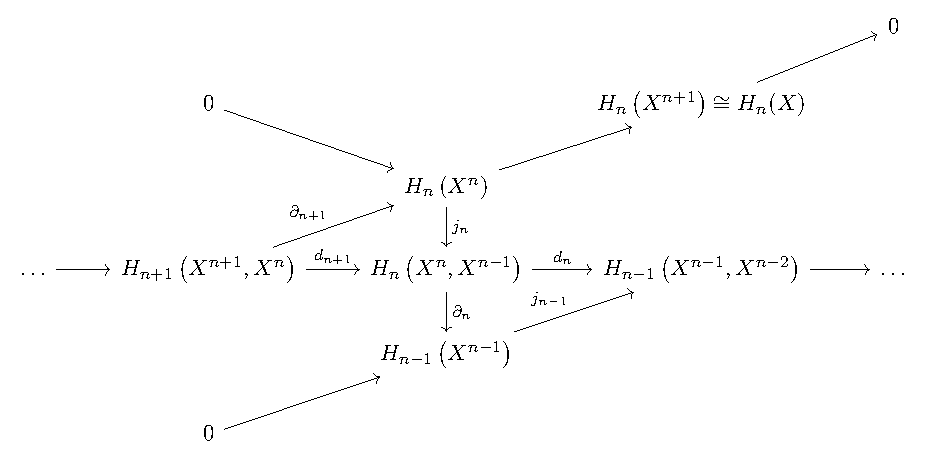
\includegraphics{lectures/0/pictures/cd_11}
    \end{center}

    Её мы получили из точных последовательностей для пар $\lr*{X^{n + 1}, X^{n}}, \lr*{X^n, X^{n - 1}}, \lr*{X^{n - 1}, X^{n - 2}}$.
    Морфизмы в нижней строчке определяются, как $d_{n + 1} \eqdef j_n \circ \partial_{n + 1}$. Нетрудно заметить, что из точности мы получаем $d_n \circ d_{n + 1} = 0$.
    Таким образом, средняя строчка диаграммы является цепным комплексом (его называют \emph{клеточным цепным комплексом для $X$}). Как мы уже замечали в доказательстве леммы выше, группа
    $H_{n}\lr*{X^n, X^{n - 1}}$~--- свободная абелева группа с базисом из $n$-мерных клеток в $X$.

    \begin{definition}
        Рассмотрим построенный выше цепной комлекс с группой $k$-мерных цепей $C_{k}^{\CW}(X) \eqdef H_{k}\lr*{X^k, X^{k - 1}}$. Гомологии этого комплекса называют
        \emph{клеточным гомологиями пространства $X$} и обозначают $H_{n}^{\CW}(X)$.
    \end{definition}

    \begin{remark}
       В самом деле, всё происходящее вполне логично~--- в случае симплициальных гомологий мы рассматриваем свободные абелевы группы, порожденные
        симплексами всех размерностей, а тут~--- клетками всех размерностей. 
    \end{remark}

    \begin{theorem}
        Пусть $X$~--- $\CW$-комплекс. Тогда имеет место изоморфизм $H_{n}^{\CW}(X) \cong H_{n}(X)$.
    \end{theorem}

    \begin{proof}
        Из точности и теоремы о гомоморфимзе мы имеем изоморфизм
        \[ H_{n}(X) \cong H_{n}\lr*{X^n}/\Im{\partial_{n + 1}}.\]
        Так как $j_n$~--- инъекция, $\Im{\partial_{n + 1}} \cong \Im{j_n \circ \partial_{n + 1}} = \Im{d_{n + 1}}$.
        С другой стороны, $\Im{j_n} \cong \Ker{\partial_n}$. Из инъективности $j_{n - 1}$ мы имеем $\Ker{\partial_n} \cong \Ker{d_n}$.
        Значит, $j_n$ индуцирует изоморфизм факторгруппы:
        \[ H_{n}(X) \cong H_{n}\lr*{X^n}/\Im{\partial_{n + 1}} \cong \Ker{d_n}/\Im{d_{n + 1}}. \]
    \end{proof}

    \begin{corollary}\label{CellularHomologyCorollary}
        Пусть $X$~--- $\CW$-комплекс, тогда:
        \begin{enumerate}
            \item $H_{n}\lr*{X} \cong 0$, если в $X$ нет $n$-мерных клеток.
            \item Если $X$~--- $\CW$-комплекс с $k$ клетками размерности $n$, то группа $H_{n}(X)$ порождена не более чем $k$ элементами.
                В самом деле, так как $H_{n}\lr*{X^n, X^{n - 1}}$~--- группа с $k$ образующими, у подгруппы $\Ker{d_n}$ никак не может быть больше образующих, а значит и в факторгруппе
                $\Ker{d_n}/\Im{d_{n + 1}}$ тоже.
            \item Если $X$~--- $\CW$-комплекс, у которого нет пар клеток в соседних размерностях, то $H_{n}(X)$~--- свободная абелева группа с базисом из $n$-мерных клеток.
        \end{enumerate}
    \end{corollary}

    \begin{example}
        Последний пункт следствия~\ref{CellularHomologyCorollary} применим, например, к $\C \mathrm{P}^n$, так как клеточная структура для $\C \mathrm{P}^n$
        имеет по одной клетке каждой четной размерности до $2n$ (действительно, это заметно из того, что $\C \mathrm{P}^n = \C^n \cup \C \mathrm{P}^{n - 1}$). Значит, клеточный цепной комплекс для $\C \mathrm{P}^n$ имеет вид:
        \[ \Z \to 0 \to \Z \to 0 \to \ldots \to 0 \to \Z \to 0 \]
        Также при помощи этого же факта можно посчитать гомологии $S^n \times S^n$.
    \end{example}

    Рассмотрим теперь подробнее клеточный оператор границы $d_n$. При $n = 1$ это легко, так как
    \[ d_1\colon H_{1}\lr*{X^1, X^0} \to H_{0}\lr*{X^0}\]
    и это просто обычное граничное отображение.

    В случае, когда комплекс $X$ связен и имеет лишь одну нульмерную клетку, $d_1 = 0$, так как
    иначе $H_{0}\lr*{X} \neq \Z$. В общем случае формула для клеточного оператора границы имеет следующий вид:

    \begin{statement}
        Имеет место равенство:
        \[ d_n\lr*{e_{\alpha}^n} = \sum_{\beta} d_{\alpha \beta} e_{\beta}^{n - 1}, \]
        где $d_{\alpha \beta}$~--- степень отображения $S^{n - 1}_{\alpha} \to X^{n - 1} \to S_{\beta}^{n - 1}$, которое является композицией
        отображения приклеивания клетки $e_{\alpha}^n$ по границе и отображения фаткоризации, стягивающего $X^{n - 1}\setminus e_{\beta}^{n - 1}$ в точку.
    \end{statement}

    \begin{proof}
        Для получения этой формулы рассмотрим такую коммутативную диаграмму:
        \begin{center}
            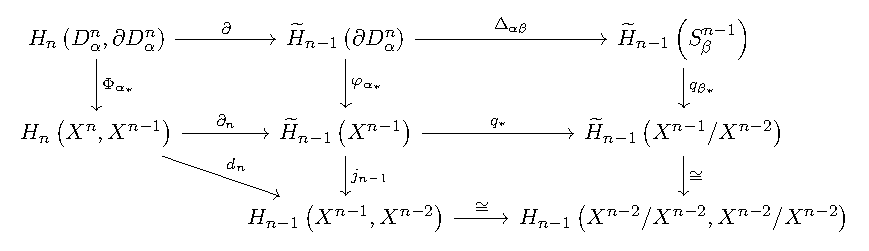
\includegraphics{lectures/0/pictures/cd_12}
        \end{center}
        Проясним, что за стрелки на ней:
        \begin{itemize}
            \item $\Phi_{\alpha}$~--- характеристическое отображение клетки $e_{\alpha}^n$, $\varphi_{\alpha}$~--- её отображение приклеивания.
            \item $q\colon X^{n - 1} \to X^{n - 1}/X^{n - 2}$~--- отображение факторизации.
            \item $q_{\beta}\colon X^{n - 1}/X^{n - 2} \to S_{\beta}^{n - 2}$~--- стягивание дополнения клетки $e_{\beta}^{n - 1}$ в точку и отождествление
            получишейся сферы с $S_{\beta}^{n - 1} = D_{\beta}^{n - 1}/\partial D_{\beta}^{n - 1}$.
            \item $\Delta_{\alpha \beta} = q_{\beta} q \varphi_{\alpha}$.
        \end{itemize}

        Отображение $\Phi_{\alpha_{*}}$ переводит образующую $[D_{\alpha}^n] \in H_{n}\lr*{D_{\alpha}^n, \partial D_{\alpha}^n}$ в образующую слагаемого
        $\Z$ группы $H_{n}\lr*{X^n, X^{n - 1}}$, соответствующего клетке $e_{\alpha}^n$ (действительно, такие клетки образуют базис $H_{n}\lr*{X^n, X^{n - 1}}$).
        Коммутативность левой половины диаграммы даёт нам, что
        \[ d_{n}\lr*{e_{\alpha}^n} = j_{n - 1}\varphi_{\alpha_{*}}\partial [D_{\alpha}^n]. \]

        Базис группы $H_{n - 1}\lr*{X^{n - 1}, X^{n - 2}}$ состоит из $(n - 1)$-мерных клеток, а отображение $q_{\beta_{*}}$~--- это проекция группы
        $\widetilde{H}_{n - 1}\lr*{X^{n - 1}/X^{n - 2}}$ (которая, как группа гомологий букета окружностей суть прямая сумма $\Z$, где каждое слагаемое соотвествует $(n - 1)$-мерной клетке)
        на её слагаемое $\Z$, соответсвующее $e_{\beta}^{n - 1}$.

        Теперь формула следует непосредственно из коммутативности правой верхней части диаграммы7
    \end{proof}


    \subsection{Гомологии поверхностей}

    В данном параграфе, пользуясь клеточными гомологиями, мы вычислим гомологии поверхностей.

    Пусть $M_{g}$~--- компактная ориентируемая поверхность с $g$ ручками. Реализуем её, как склейку $4g$-угольника:
    \begin{center}
            \begin{tikzpicture}
            \node at (0,0){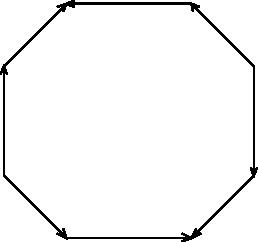
\includegraphics{lectures/0/pictures/pic_5}};
            \node at (-2.3, 0){\small \( a \)};
            \node at (2.3, 0){\small \( c \)};
            \node at (-1.75, 1.6){\small \( b \)};
            \node at (0, 2.2){\small \( a \)};
            \node at (0, -2.2){\small \( c \)};
            \node at (1.75, 1.6){\small \( b \)};
            \node at (1.75, -1.6){\small \( d \)};
            \node at (-1.75, -1.6){\small \( d \)};
            %	\draw[opacity=0.7] \foreach \x in {-4,...,5} {
	   (\x cm, 0.1) -- (\x cm, -0.1) node[below]{\tiny \x}
	   (\x cm - 0.5cm, 0.08) -- (\x cm - 0.5cm, -0.08)
	   \foreach \t in {1,2,3,4,6,7,8,9} {
	      (\x cm - 0.1 * \t cm, 0.055) -- (\x cm - 0.1 * \t cm, -0.055)
	   }
	};
	\draw[opacity=0.7,rotate=90] \foreach \x in {-3,-2,-1,1,2,3,4} {
	   (\x cm, 0.1) -- (\x cm, -0.1) node[right]{\tiny \x}
	   (\x cm - 0.5cm, 0.08) -- (\x cm - 0.5cm, -0.08)
	   \foreach \t in {1,2,3,4,6,7,8,9} {
	      (\x cm - 0.1 * \t cm, 0.055) -- (\x cm - 0.1 * \t cm, -0.055)
	   }
	};
;
            \end{tikzpicture}
    \end{center}

    Тогда в её клеточном разбиении:
    \begin{itemize}
        \item 1 двумерная клетка, приклеенная по произведению коммутаторов $[a_1, b_1] \ldots [a_{g}, b_{g}]$.
        \item $2g$ одномерных клеток.
        \item 1 нульмерная клетка.
    \end{itemize}

    Значит, цепной клеточный комплекс для $M_g$ будет иметь вид:
    \[ 0 \to \Z \xrightarrow{d_2} \Z^{2g} \xrightarrow{d_1} \Z \to 0 \]

    Так как комплекс связен и имеет лишь одну нульмерную клетку, $d_1 = 0$. Кроме того, каждое ребро $[a_1, a_2], \ [a_{g}, b_{g}]$
    появляется в произведении коммутаторов вместе со своим обратным, а значит, $\Delta_{\alpha \beta}$ гомотопны постоянным отображениям, из чего следует, что $d_{2} = 0$.

    Таким образом, мы имеем
    \[ H_{k}\lr*{M_{g}} = \begin{cases} \Z, \quad k = 0 \text{ или } k = 2, \\ \Z^{2g}, \quad k = 1 \\ 0, \quad \text{иначе}\end{cases}\]

    Теперь вычислим гомологии неориентируемой замкнутой поверхности рода $g$. Она имеет такую клеточную структуру:
    \begin{itemize}
        \item Одна нульмерная клетка.
        \item $g$ одномерных клеток.
        \item Одна двумерная клетка, приклеенная по слову $a_{1}^{2}\ldots a_{g}^{2}$.
    \end{itemize}
    Тогда клеточный цепной комплекс имеет вид:
    \[ 0 \to \Z \xrightarrow{d_2} \Z^{g} \xrightarrow{d_1} \Z \to 0 \]
    Аналогично предыдущему разу, $d_{1} = 0$, а вот $d_{2}$ задаётся уравнением
    \[ d_{2}(1) = (2, \ldots, 2), \]
    так как  каждое ребро $a_i$ появляется в слове приклеивания двумерной клетки со степенью 2, а это значит, что каждое отображение
    $\Delta_{\alpha \beta}$ гомотопно отображению степени 2. Значит, $d_{2}$ инъективно и
    \[ H_{2}(N_{g}) = 0. \]

    Выберем в $\Z^{g}$ такой базис: $(1, 0, \ldots, 0), (0, 1, 0, \ldots, 0), \ldots, (0, \ldots, 1, 0), (1, 1, \ldots 1)$. Тогда нетрудно заметить, что
    \[ H_{1}\lr*{N_{g}} \cong \Z^{g - 1} \oplus \Z/2\Z. \]

    \subsection{Пространства Мура}

    Допишу позже вместе с пространствами Эйленберга-Маклейна.

    \subsection{Теорема о вложении дисков и сфер}

    Напомним, что топологическое вложение~--- гомеоморфизм на образ.

    \begin{theorem}
        Пусть $h\colon D^k \to S^n$~--- вложение. Тогда
        \[ \widetilde{H}_{i}\lr*{S^n \setminus h\lr*{D^k}} = 0 \ \forall i. \]
        Кроме того, если $h\colon S^k \to S^n$~--- вложение (и $k < n$), то
        \[ \widetilde{H}_{i}\lr*{S^n \setminus h\lr*{S^k}} = \Z, \ i = n - k - 1 \text{ и } 0 \text{ иначе. }\]
    \end{theorem}
    \begin{proof}
        Проведём индукцию по $k$. Случай $k = 0$ тривиален:
        \[ S^n \setminus h\lr*{D^0} = \R^n. \]
        Теперь докажем индукционный переход от противного. Рассмотрим покрытие нашего пространства двумя множествами:
        \[ A = S^n \setminus h\lr*{I^k \times \left[0, \frac{1}{2}\right]}, \quad B = S^n \setminus h\lr*{I^k \times \left[\frac{1}{2}, 1\right]}. \]
        Заметим, что $A \cup B = S^n \setminus \lr*{h\lr*{I^k \times \left[0, \frac{1}{2}\right]} \cap h\lr*{I^k \times \left[\frac{1}{2}, 1\right]}} = S^n \setminus h\lr*{I^k \times \frac{1}{2}}$ и
        \[ \widetilde{H}_{i}(A \cup B) \cong \widetilde{H}_{i}\lr*{S^n \setminus h\lr*{I^k \times \frac{1}{2}}} = 0,\]
        по индукционному предположению.
        Напишем теперь точную последовательность Майера-Вьеториса (\ref{Mayer–Vietoris_sequence}):
        \[ \ldots \to H_{n}(A \cap B) \to H_{n}(A) \oplus H_{n}(B) \to H_{n}(X) \to H_{n - 1}(A \cap B) \to \ldots \]
        \[\ldots \to  H_{n}\lr*{S^n \setminus h\lr*{I^{k + 1}}} \to H_{n}(A) \oplus H_{n}(B) \to \underbrace{H_{n}\lr*{S^n \setminus h\lr*{I^k \times \frac{1}{2}}}}_{\cong 0} \to H_{n - 1}\lr*{S^n \setminus h\lr*{I^{k + 1}}} \to \ldots \]
        \[ \]
        значит если в $\widetilde{H}_{i}\lr*{A \cap B} = \widetilde{H}_{i}\lr*{S^n \setminus \lr*{I^{k} \times I}}$ есть ненулевой класс $a$, его образ $(a, -a)$ в  $\widetilde{H}_n(A) \oplus \widetilde{H}_n(B)$ будет ненулевым, а значит, в  $\widetilde{H}_{i}(A)$ или $\widetilde{H}_{i}(B)$  тоже будет ненулевым.
        Далее мы можем также разбить на две части интервал в $A$ или в $B$ (в зависимости от того, где не ноль) и проделать всё полностью аналогично.
        Таким образом мы получим последовательность вложенных интервалов $I_n$ таких, что
        \[ \widetilde{H}_{i}\lr*{S^n \setminus h\lr*{I^{k} \times I_n}} \neq 0, \ a \in \widetilde{H}_{i}\lr*{S^n \setminus h\lr*{I^{k} \times I_n}}. \]
        Тогда, если $p = \bigcap I_n$, то по индукционному предположению
        \[ \widetilde{H}_{i}\lr*{S^n \setminus h\lr*{I^k \times p}},  \]
        то есть $a$ представляет ноль в этих гомологиях. Но это означает, что он является чьей-то границей, но тогда он является границей и в допредельном случае, что даёт нам противоречие.

        Докажем теперь второй пункт. Представим сферу ввиде объединения двух дисков (полусфер):
        \[ S^k = D^k_{+} \cup D^k_{-}, \quad D_{-}^{k} \cap D_{+}^{k} = S^{k - 1}. \]
        тогда $S^n \setminus h\lr*{S^k} = S^n \setminus h\lr*{D^{k}_{+} \cup D^{k}_{-}} = S^n \setminus h\lr*{D_{-}^k} \cap S^n \setminus h\lr*{D_{+}^k}$.
        Запишем опять точную последовательность Майера-Вьеториса~\ref{Mayer–Vietoris_sequence}, полагая
        \[ A = S^n \setminus h\lr*{D_{+}^k}, \quad B = S^n \setminus h\lr*{D_{+}^k}. \]:
        \[ \ldots \to H_{i}\lr*{S^n \setminus h\lr*{S^{k}}} \to \underbrace{H_{i}\lr*{S^n \setminus h\lr*{D^k_{-}}}}_{= 0} \oplus \underbrace{H_{i}\lr*{S^n \setminus h\lr*{D^k_{+}}}}_{= 0} \to H_{i}\lr*{S^n \setminus h\lr*{S^{k - 1}}} \to \ldots  \]
        Нулевые элементы в точной последовательности у нас их первого утверждения теоремы. Теперь видно, что мы можем вести индукцию по $k$.
    \end{proof}

